%\documentclass[handout]{beamer}
\documentclass[10pt]{beamer}
%for(int i=0; i<n; i++){\documentclass[10pt,handout]{beamer}
\usepackage[spanish]{babel}
% % \usepackage[backend=biber, style=authoryear-icomp]{biblatex}
\resetcounteronoverlays{exx}
\usepackage{mdframed}
\usepackage{tikz}
\usepackage{blindtext}
\usepackage{tipa}
% \usepackage{cgloss4e}
% \usepackage{gb4e}
% \usepackage{qtree}
\usepackage{cancel}
\usepackage{wrapfig}
\usepackage{soul}
\usepackage{enumerate}
\usepackage{longtable}
\graphicspath{ {./figures/} } % declaramos donde estan las imagenes
\usepackage[labelformat=simple]{subcaption} % para varias imagenes juntas
\renewcommand\thesubfigure{(\alph{subfigure})}
\usepackage[utf8]{inputenc}
\usepackage{amsmath}
\usepackage{amsfonts} % simbolos como el I de matriz identidad
\usepackage{bm}
\usepackage{graphicx} % paquete para ver imagenes
\usepackage{setspace}
\usepackage[T1]{fontenc}
\usepackage{parskip}
\usepackage{color}
\usepackage{framed}

\usetheme{Copenhagen}
\definecolor{frenchblue}{rgb}{0.0, 0.45, 0.73} % ESTE!!!!

\setbeamercolor{block body}{bg=frenchblue!50}
\setbeamercolor*{structure}{fg=frenchblue,bg=blue}
\setbeamercolor{normal text}{fg=black}
\setbeamercolor{frametitle}{bg=black}
\setbeamertemplate{frametitle}[default][center]
\setlength{\parskip}{12pt}
\useoutertheme{infolines} % me comia mucho espacio de la otra fgorma
\makeatother
\setbeamertemplate{footline}
{
  \leavevmode%
  \hbox{%
  \begin{beamercolorbox}[wd=.3\paperwidth,ht=2.25ex,dp=1ex,center]{author in head/foot}%
    \usebeamerfont{author in head/foot}\insertshortauthor
  \end{beamercolorbox}%
  \begin{beamercolorbox}[wd=.6\paperwidth,ht=2.25ex,dp=1ex,center]{title in head/foot}%
    \usebeamerfont{title in head/foot}\insertshorttitle
  \end{beamercolorbox}%
  \begin{beamercolorbox}[wd=.1\paperwidth,ht=2.25ex,dp=1ex,center]{date in head/foot}%
    \insertframenumber{} / \inserttotalframenumber\hspace*{1ex}
  \end{beamercolorbox}}%
  \vskip0pt%
}
\makeatletter
\setbeamertemplate{navigation symbols}{}
%\setbeameroption{show notes}
\setbeameroption{hide notes}
\renewcommand{\CancelColor}{\color{red}}

\usepackage{hyperref}

\title[RISC II]{Presentación RISC II}
\author[Matias Mazzanti]{Matias Mazzanti}


\institute{DC-UBA}
\date{05 de Septiembre de 2022}

\titlegraphic{
\includegraphics[,height=2cm,keepaspectratio]{../logo.pdf}     }
%\logo{
\includegraphics[height=2.5cm]{logo.PDF}}

\begin{document}

\begin{frame}

\maketitle

\end{frame}

% cuál es tu background que estuviste haciendo y qué querés hacer
% Con quién vas a trabajar en los planes
% un poquito de cuál es la idea del doctorado aunque todavía este verde

\section{Presentaci\'on}
\begin{frame}
\frametitle{Introducción}

\begin{itemize}
  \item Licenciado en Ciencias de la Física.
  \item Alumno doctoral de Esteban Mocskos: Laboratorio Interdisciplinario de Computación de Alto Rendimiento. UBA.
  \item Tema doctoral: Soporte en Hardware para FHE (Fully Homomorphic Encryption).
\end{itemize}

\end{frame}



\begin{frame}
\frametitle{Introducción}
\begin{figure}[h!]
    \centering
    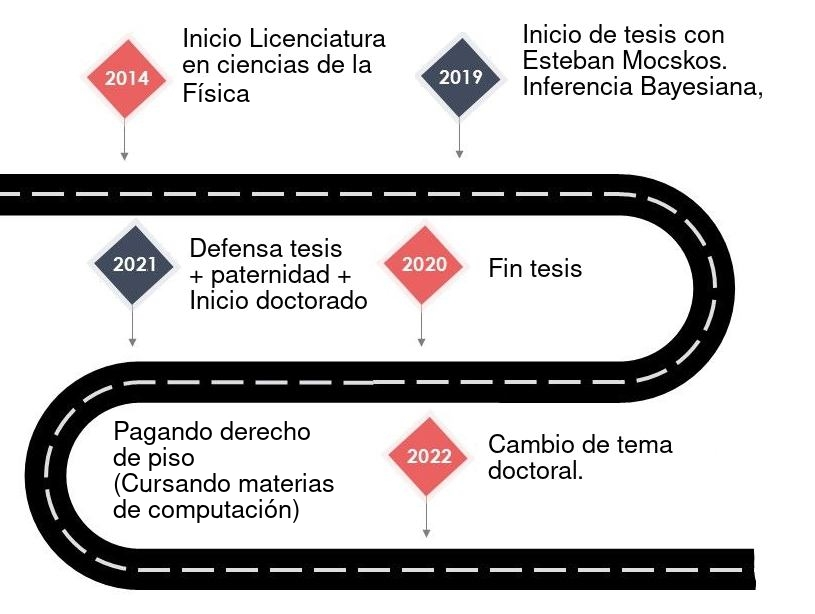
\includegraphics[scale=0.3]{road.jpg}
\end{figure}
\end{frame}


\begin{frame}
\frametitle{Origenes y tesis}

 Durante la Lic Física me acerqué a la computación (materias optativas).
\begin{columns}
    \column{0.5\textwidth}
\vspace{0.5cm}

Tesis dentro del departamento de computación de la UBA.
\vspace{0.5cm}

Estimaciones Bayesianas de la habilidad en jugadores del juego de mesa de Go.

\vspace{0.5cm}
Se propuso una mejora en el sistema de rankeo para plataformas online.
    \column{0.5\textwidth}
\begin{figure}[h!]
    \centering
    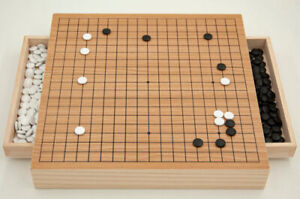
\includegraphics[scale=2.]{go.jpg}
\end{figure}
\end{columns}
\end{frame}

\begin{frame}
\frametitle{Doctorado}
Propuesta original: Continuar el tema de la tesis utilizando el modelo de estimación y buscar su paralelización mediante GPU.

La paralelización para el modelo no se justificaba $\rightarrow$ utilizar el modelo para responder otras preguntas.

Modelar y estudiar el aprendizaje humano.

El camino que tomó el doctorado  no me convenció $\to$ cambio de planes.



\end{frame}

\begin{frame}
\frametitle{Cambio Doctorado}

\begin{columns}
    \column{0.5\textwidth}
        Director: Esteban Mocskos UBA
        \vspace{0.3cm}

        Codirector: Augusto Vega IBM

        \vspace{0.3cm}
        Fully Homomorphic Encryption (FHE).

        \vspace{0.3cm}
        Operar \textbf{directamente} con datos encriptados (sin necesidad de desencriptar).


    \column{0.5\textwidth}
\begin{figure}[h!]
    \centering
    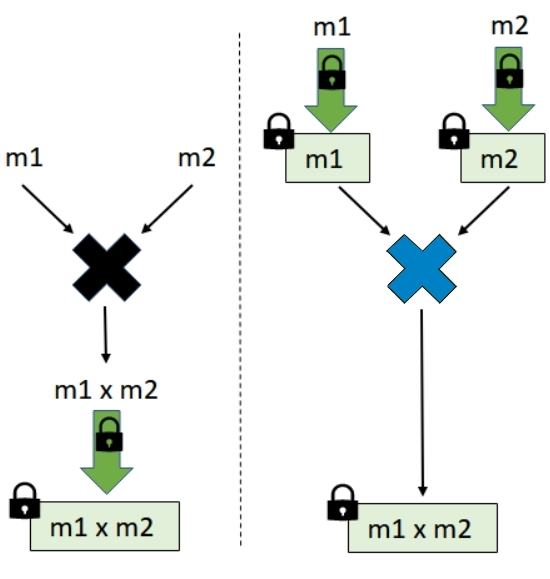
\includegraphics[scale=0.19]{mult.jpg}
\end{figure}
\end{columns}


Ej: Lograr procesar remotamente con machine learning sin revelar los datos.

Potencialmente con mucha utilidad para uso de cloud computing.

Actualidad: muy lento para uso real.

\begin{mdframed}[backgroundcolor=frenchblue!20]\centering
  Acelerar mediante hardware.
\end{mdframed}

\end{frame}


%Complejidad de FHE,

%Por que se requiere aceleracion por hardware

%Costos computacionales

%Limites


\begin{frame}
\frametitle{FHE}
Requierimientos FHE:
\begin{itemize}
  \item Homomorfismo en la suma y multiplicación.
  \item Ilimitada cantidad de operaciones.
  \item Tiempos razonables
\end{itemize}

Problemas:
\begin{itemize}
  \item No todo esquema es homomorfico en ambas operaciones. Ej RSA permite solo multiplicación (Partially HE).
  \item La mayoría de esquemas utilizan \texttt{Learning With Errors} (LWE). Aumentando su error por cada operación.
  \item Los esquemas actuales tienen un costo muy grande por cada operación: orden del segundo.
\end{itemize}




\end{frame}

\begin{frame}
\frametitle{Boostraping}
Gentry $\to$ \texttt{Boostraping}: reducir el error luego de una operación.

El boostraping es uno de los principales cuellos de botella de FHE.
\begin{figure}[h!]
    \centering
    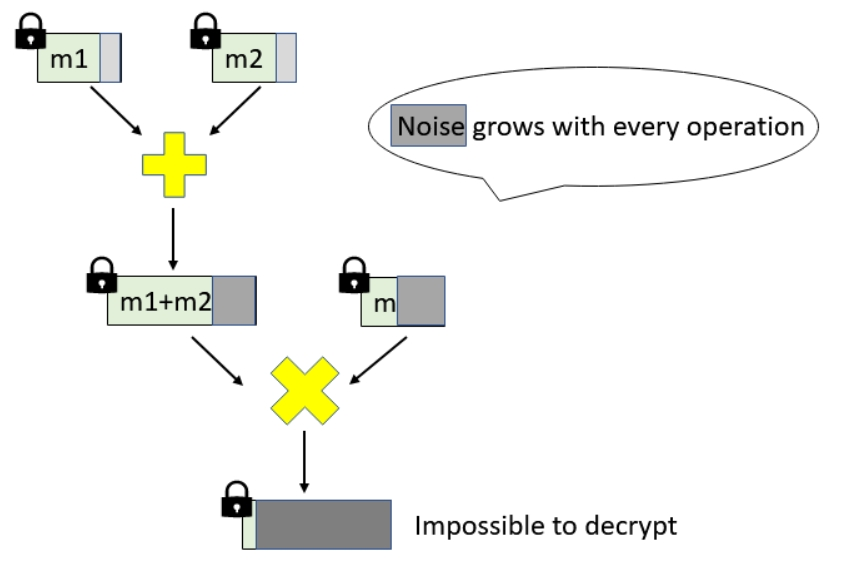
\includegraphics[scale=0.3]{multNoise.jpg}
\end{figure}
\end{frame}
\begin{frame}
\frametitle{}
  \begin{figure}[h!]
      \centering
      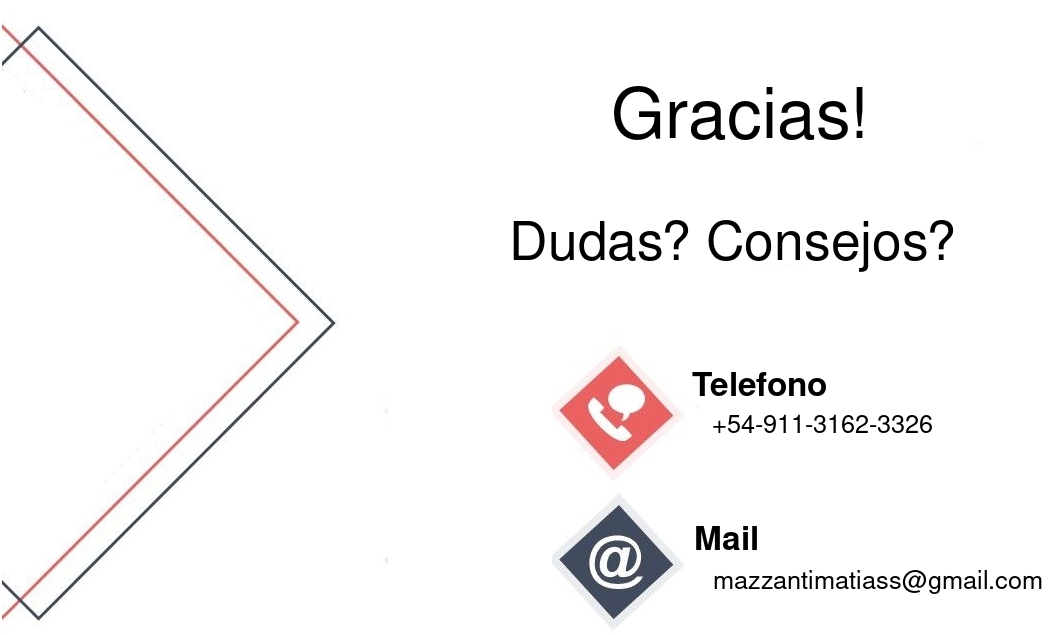
\includegraphics[scale=0.3]{agradecimientos.jpg}
  \end{figure}
\end{frame}
\end{document}
